\documentclass{article}

\usepackage{nips_2018_author_response}

\usepackage[utf8]{inputenc} % allow utf-8 input
\usepackage[T1]{fontenc}    % use 8-bit T1 fonts
\usepackage{hyperref}       % hyperlinks
\usepackage{url}            % simple URL typesetting
\usepackage{booktabs}       % professional-quality tables
\usepackage{amsfonts}       % blackboard math symbols
\usepackage{nicefrac}       % compact symbols for 1/2, etc.
\usepackage{microtype}      % microtypography
\usepackage{wrapfig}
\usepackage{bm}
\usepackage{xspace}

%\usepackage[subtle]{savetrees}

\usepackage[colorinlistoftodos,prependcaption,textsize=tiny]{todonotes}


% Our model

\newcommand{\ourModel}{\textsc{Electro}\xspace}
\newcommand{\ourModelIR}{\textsc{Electro-Lite}\xspace}
\newcommand{\ourModelR}{\textsc{Electro}\xspace}

\widowpenalty=100000000


\begin{document}

%% ============================================
%% ========= Intro Section  ===================
%% ============================================


\begin{wrapfigure}{r}{0.6\textwidth}
\centering
\vspace{-1pt}
  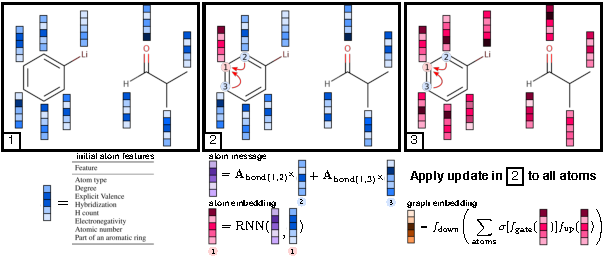
\includegraphics[width=10cm]{graph_nn.pdf}
  \vspace{-18pt}
 \caption{New image we propose putting in Section 3 of the paper to clarify the overall workflow for forming node and graph embeddings via a message passing framework (following the approaches in [9-10]).}
 \label{fig:new-diagram}
 \vspace{-5ex}
\end{wrapfigure}

We would like to thank all reviewers for their thoughtful comments. 
%Thank you for taking the time to review our paper. 
%\todo[]{Some changes to fig: a. missing vectors for some atoms, b. make super explicit that A shared by changing sub index to single and double bond, c. use table to refer to explicitly refer to Table 1 in SM for more details, d. make it clear that boxes (2) and (3) happen multiple times; e. Change the sum to be over mathcal A'}
% We are grateful for your suggestions about improving the description of the model. We therefore have made a few changes to section 3 to improve clarity.
% In particular, we add a step-by-step description of the workflow and a new diagram, Figure \ref{fig:new-diagram}, to provide background on GGNNs and how these can be used to provide graph and node embeddings. 
% In addition we have brought out of the supplementary material some details on more specific architecture choices and to have space to do so, we are grateful to R2's suggestion to move the more technical details of section 4 into the appendix.
%To the more specific individual comments we respond to each reviewer below.
%We respond to each reviewer below.
Our responses are below (new experiments are marked with 
\includegraphics[width=0.3cm]{testtube.png}
):
%% ============================================
%% ========= Reviewer 1  ======================
%% ============================================

\vspace{-5pt}
\paragraph{Reviewer 1}

%\emph{(2) Why the present method is expected to perform better than WLDN in product prediction?}
\emph{[..(1) workflow..]} 
Thank you for this. We will make the following changes: add a step-by-step description of GGNNs as shown in Figure~\ref{fig:new-diagram}, bring out of the appendix information on architectures and workflow. 

\emph{[..(2) why better than WLDN?..]}
Our argument is that \ourModel is much closer to the underlying physical reality of reaction mechanisms (sequential electron redistribution steps), so it outperforms WLDN by encoding needed compositional inductive biases. 
% Alongside this, we believe that (1) the interpretability provided by \ourModel by modeling the mechanism steps and (2) the avoidance of having to set up a somewhat more fragmented ML pipeline of predict-then-rank steps are also advantageous.% features of our model.
We believe avoiding the WLDN more fragmented ML pipeline of predict-then-rank steps is also advantageous.  % features of our model. 


%\emph{(3) How the present model compares to WLDN and seqtoseq in terms of runtime.}

\includegraphics[width=0.3cm]{testtube.png} \emph{[..(3) runtime comparison..]}
For predicting products %, using a beam search width of 10, 
\ourModel takes $0.337$ seconds, versus $0.034$s for WLDN [5] and $0.025$s %\footnote{As no code is available for this paper we quote their stated time.} 
for the Seq2Seq model (quoting their stated time) [14, \S6.2]. 
%\todo[]{Check wldn timings as they give 50ms in paper. Maybe they include the initial rdkit time.}
 However, the majority of the time for \ourModel ($0.193$s) is used within RDKit to create intermediate molecules and their features, an operation that is not currently parallelized across the different beams; only $0.044$s is used given the features to compute the action probabilities.
  At test time we take advantage of the embarrassingly parallel nature of the task to parallelize across test inputs. 
   Finally, to compute the log likelihood of a reaction (with access to the intermediate steps), it only takes $0.007$s for \ourModel. %\todo[]{Can also add the fact we have less parameters.}


%The timings of the models are given in Table \ref{table:timings}. We shall include these in the paper.
% For Electro we use a beam width of ten. 
% Although the overall time is greater than the others, only 0.044 secs is used to compute the probabilities and the majority of the time (0.193 secs) is used using RDKIT to create intermediate molecules or derive features from them, an operation that is not currently parallelized across the different beams. 
% Instead as the whole predict operation for Electro only takes 0.428 secs on a CPU we take advantage of the embarrassingly parallel nature of the task across different reaction predictions when running Electro on the test set.
% If we are interested in only computing the log likelihood of a reaction (and so have access to all the intermediate steps), this takes 0.007 secs on a GPU for Electro.
% 
%\begin{table}[h]
%  \caption{Time taken in seconds to predict product from the initial reactant and reagent molecules.
%  These have been run on a NVIDIA 1080 GPU, with the mean time taken over the first 500 items of the test set.
%  * As no code is available for [14] we instead report the timings given in Section 6.2 of their paper.
%  }
%  \label{table:timings}
%  \centering
%  \begin{tabular}{llll}
%    \toprule
%    & Electro (Ours) & WLDN [5] & Seq2Seq [14]  \\
%    \midrule
%    Timing (secs) & 0.337   & 0.034 &  0.025*     \\
%    \bottomrule
%  \end{tabular}
%\end{table}



%% ============================================
%% ========= Reviewer 2  ======================
%% ============================================
\vspace{-5pt}
\paragraph{Reviewer 2}

\includegraphics[width=0.3cm]{testtube.png} \emph{[i]}
The motivation of only including reagent context at the start is that choosing the first entry in the electron path is often the most challenging decision, and that action steps after this have access to the previous atom as context, making it an easier task.
%Qualitatively, when running Electro-lite on the separate validation set we would see that the model often had the most errors on the first step, and that after picking this first step the next stages would often be correctly predicted.
We have tested a version of \ourModel where reagent information is fed in as context at each step. 
On the mechanism prediction task (Table 1) this gets a slightly improved top-1 accuracy of $78.4\%$ ($77.8\%$ before) but a similar top-5 accuracy of $94.6\%$ ($94.7\%$ before). On the reaction product prediction task (Table 2) we get $87.5\%$, $94.4\%$ and $96.0\%$ top-1, 3 and 5 accuracies ($87.0\%$, $94.5\%$ and $95.9\%$ before).

\emph{[ii \& iv]}
Thanks. We will add details on GGNNs via Figure~\ref{fig:new-diagram}, and move architecture choices from the supplementary.
%One of the nice features of the approach is that we can easily break down the loss (or equivalently the negative log likelihood) of each prediction our model makes. 
%Empirically we found that Elctro-lite on the first 500 items of the validation set obtained a median loss of 0.209 on predicting where to start, whereas the first add step (when applicable) would contribute a median loss of 0.002, highlighting the sometimes much poorer performance of this module.
%When testing Electro, its initial select module would get a median loss of 0.023, showing that the addition of reagents, greatly improves the prediction of this task.

\emph{[iii]} 
Sorry for the confusion here. In eq 4, $\mathbf{H}_m$ should be $\mathbf{H}_{\mathcal{M}_t}$. We apologize for this typo.
In eq 2 $\mathcal{A}’$ is the set of all atoms in the graphs under consideration. For example, when forming the reagent context vector this will be only the reagents.
The dependency on $a_{t-1}$ is due to the changes in the molecular graph, caused by action $a_{t-1}$. 
To clarify this, we will add equations for each of our predictors: $f_\textrm{start}$, $f_\textrm{add}$, $f_\textrm{remove}$ (which are currently in the supplement).

\emph{[v]} 
We thought a lot about how to compare with [6-7], but
 ultimately we decided we were unable to because:
  1.These methods, as they currently stand, cannot run on all the elements present in USPTO [6, p.2528], [7, p.2214] and, furthermore, require access to the (unknown) reaction conditions. 
 2. We cannot run our method on their data as the link to their data is missing atom information, and they did not respond to our emails asking for their code or data. 


\includegraphics[width=0.3cm]{testtube.png} \emph{[vi]} We trained WLDN [5] (using code from the authors) on our filtered training dataset.
 We found it achieved top-1, top-3 and top-5 accuracies of $83.1\%$, $91.5\%$ and $92.7\%$, which is worse than \ourModel. 
 Thus the improvements of \ourModel are not due to a more specialized training task.
  
\emph{[vii]}
 We politely disagree here.
  We think it is completely surprising that the model is able to pick up subtle chemical trends (e.g., single atomic changes) without being explicitly trained on this task.
   We think an experiment like this may give additional confidence to a chemist, %that our model has learned reaction prediction, 
   as this experiment resembles exam questions for organic chemistry students. %\todo[]{could say we will motivate this reasoning better}
 
\emph{[viii]}
We believe this work advances two novel directions for future research: 
%1. We observe that reactions are essentially stepwise graph-editing procedures. 
 %It’s fruitful to model it this way precisely because it sets the stage for models that work on more general types of chemical reactions.
  1. We think that setting up reactions as stepwise graph-editing procedures can be extended with suitable changes to a greater class of reactions.
%It also potentially can be applied on graph editing based applications outside the domain of chemistry.
 2. More broadly, there is a significant amount of structure and powerful abstractions developed in chemistry, that we as ML researchers can take advantage of, to aid the interoperability, interrogation and the improvement of  models;
and we believe \ourModel is a motivating and successful example of how this can be done.

%  2. More broadly, there is a significant amount of structure and powerful abstractions developed in chemistry, that we as ML researchers can take advantage of, to aid the interoperability, interrogation and the improvement of  models;
%\ourModel is an example of such a model taking advantage of the powerful abstractions of reaction mechanisms.
%%and by visualizing these mechanisms we can show that it does the same sorts of things that organic chemistry students learning reactions do.
%We hope that this in turn encourages a direction of research in which existing useful abstractions and tools in application areas are harnessed when developing new ML algorithms.




 
 
 



%% ============================================
%% ========= Reviewer 3  ======================
%% ============================================
\vspace{-5pt}
\subparagraph*{Reviewer 3}
%\emph{"On one hand, theis paper includes several modelling ideas that might have the potential to indeed advance the field. On the other hand, from a chemical perspective the model is still rather limited, since only topological molecule descriptors are used, neglecting the influence of conformational changes."}
%\emph{Point under EVALUATION, on significance)}
\emph{[..on significance..]}
Thank you for recognizing and commending our modelling ideas. We agree conformational change information is certainly useful and underused in work at ML venues for reaction prediction. We aim to consider this in future work.
That said, in this work, our purely topological model is harnessing the extremely powerful arrow-pushing abstraction. 
It allows chemists to make very quick, but accurate predictions without doing any quantum simulations, and to understand relations between reaction classes, which is not possible using quantum mechanics alone. \looseness=-1

\emph{[..on clarity..]}
Thanks, we will move architecture choices from the supplementary and include Figure \ref{fig:new-diagram} for more detail.


\end{document}
